\documentclass[]{standalone}

\usepackage{mathptmx}
\renewcommand{\familydefault}{\rmdefault}
%\usepackage[T1]{fontenc}
%\usepackage[latin9]{inputenc}
\usepackage{siunitx}
\usepackage{array}
\usepackage{amsmath}
\usepackage{ifthen}
\usepackage{pgfplots}
\pgfplotsset{compat=1.18}
%\usepackage[]{gnuplottex}
\usepackage{titling, graphicx}
\usepackage{tikz}
\usepackage{upgreek}
\usepackage{amsmath,amsthm}
\usepackage{strtikz}
\usepackage{circledsteps}
\usepackage{nicefrac}
\usepackage{tikz-dimline}
\usepackage{latexcolors}
\usepackage{pdfrender}
\usepackage{upgreek}
\usepackage{bigints}
\usetikzlibrary{shapes,arrows.meta,intersections,graphs,graphs.standard}
\usetikzlibrary{bending, math,fit}
\usetikzlibrary{calc,intersections,through,backgrounds}
\usetikzlibrary{decorations.markings,decorations.pathmorphing, decorations.pathreplacing}
\usetikzlibrary{patterns}


\begin{document}
\def \fsize {\tiny}
\begin{tikzpicture}
\bilinear[startx = 0cm,
starty = 0cm,
yield displacement = 1cm,
yield force = 2cm,
maximum displacement = 5cm,
maximum force = 2.5cm,
axis space = 1.0cm,
mode = 8,
x-axis label = {$D$},
y-axis label = {$F$},
kp text = $k_\text{p}$,
ks text = $k_\text{s}$,
fy text = $f_\text{y}$,
dy text = $d_\text{y}$,
mark yield point = 1,
fmax text = $f_\text{m}$,
dmax text = $d_\text{m}$,
mark max point = 1,
axis line thickness = 1pt,
line thickness = 1pt,
show axes labels = 1,
show stiffness = 1,
show arrows = 0,
show line arrows = 1,
arrow length = 6pt,
arrow width = 4pt,
show top border = 1,
show bottom border = 1,
border line color = red,
border line thickness = 1pt,
border line dash = dashed,
border line opacity=0.5,
show qy = 1,
qy text = {$q_\text{y}$},
show shade = 1,
shade color = blue,
shade opacity = 0.25,]
%\draw (0,0) -- (1cm,1cm);
\end{tikzpicture}
\end{document}